\chapter{Optimization with Gradient Descent}\label{gd}
All throughout Machine Learning gradient descent and variations of it are used for optimization. Gradient descent is vital for my work. As such I will I will briefly explain what it is and how it is relevant to my work.

\section{What is Gradient Descent?}\label{gd:what_is_it}
In essence gradient descent is an algorithm used to find local minima of differentiable functions. It can be thought of as starting at a point on the function graph and walking down hill until one reaches a minimum. Gradient descent works by differentiating a function at some point in order to obtain a slope, and then moving in the downwards direction of that slope. Gradient descent is done in steps. If $f(\theta)$ is a differentiable function, then one gradient descent step is:

\begin{equation}\label{Graident_Descent:basic_update}
    \theta \leftarrow \theta - \alpha \cdot \frac{\partial}{\partial \theta}f(\theta)
\end{equation}

\noindent
\\ The \textit{step size} $\alpha$ is introduced to control the magnitude of the descent step. The gradient descent algorithm consists of performing these steps iteratively until the current value (in the above case $\theta$) is sufficiently close to the actual local minimum. Performing 10 gradient descent steps on the function $f(\theta) = \theta^2$ and a starting value of $\theta = 3$ with various values for alpha looks as follows:

\begin{figure}[ht]
    \centering
    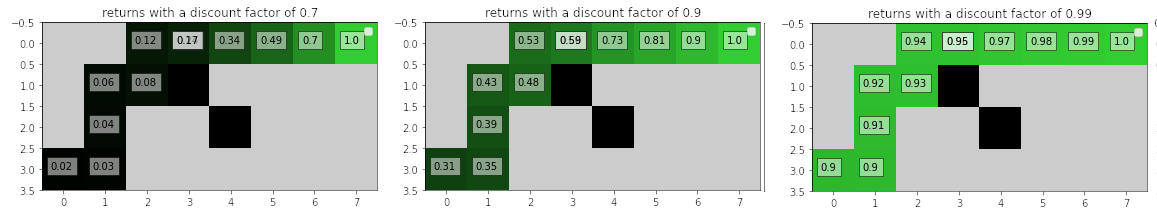
\includegraphics[width=\linewidth]{figures/grid_world_discount_factors.png}
    \caption{Gradient Descent on $f(\theta) = \theta^2$}
    \label{fig:UNO}
\end{figure}

\noindent
\\ As can be clearly seen here smaller step sizes lead to more accurate results. Too large a step size may even lead to divergence. However, if the step size is too small, it may take very long to reach a local minimum. Gradient descent functions in the exact same way if $\theta$ is a vector. In that case the update step becomes:

\begin{equation}\label{Graident_Descent:basic_update_vector}
    \theta \leftarrow \theta - \alpha \cdot \nabla_\theta f(\theta)
\end{equation}

\subsection{Gradient Descent on functions which take unknown variables}\label{gd:random_var}
Gradient Descent can also be used to minimize function parameters when unknown variables are in the mix, and the goal is to find parameters which lead to minimal function values for most parameters. Say $f(x, \theta)$ is the function we are performing gradient descent on, $\theta$ is a vector of parameters we are trying to optimize, and $x$ is sampled from a distribution. We can perform gradient descent steps which are close to optimal, by calculating the gradients $\nabla_\theta f(x, \theta)$ for $n$ number of samples of $x$, averaging them, and performing a gradient descent step on that average. The more samples of $x$ we have the more accurate the direction and magnitude of the step are going to be going to be.

\subsection*{Gradient Ascent}\label{gd:gradient_ascent}
As the name implies gradient ascent is the exact opposite of gradient descent. Instead of trying to find the local minimum of a function, when performing gradient ascent we are trying to find the local maximum of a function. Gradient Ascent is identical to performing Gradient Descent on the negative derivatives. 

\section{How is Gradient Descent relevant to Reinforcement Learning?}\label{gd:relevance}
In the previous chapter we have established that policies are functions which take actions and produce probability distributions over a set of actions. They may also be parameterized. One very common way of optimizing policies is to define a function $J(\theta)$, which measures agent performance \citepg{312}. This function is dependant on, and differentiable with respect to, the policy parameters $\theta$. Gradient Descent or Ascent (which one we use is dependant on if the performance measuring function treats lower or larger values as better) can then be used to optimize $\theta$. I will present one such function, in chapter \ref{chap:policy_gradient}. Gathering a set of agent-environment interactions, using the rewards received in them in a performance measuring function which depends on the policy parameters, and then using a variation on Gradient Descent to optimize those parameters, is the method i use to train an agent in this thesis. This can be represented in an abstract algorithmic fashion:

\begin{algorithm}[H]
\SetAlgoLined
 initialization\;
 \Repeat{agent performance suffices}{
  \For{$t \in 0, \dots, n$}{
   Get state $S_t$\;
   Take action $A_t$ sampled from $\pi(a|s,\theta)$\;
   Receive reward $R_t$\;
  }
  Compute gradients of performance function based on rewards w.r.t. $\theta$\;
  update $\theta$ with Gradient Descent;
  
 }
 \caption{Reinforcement Learning With Gradient Descent}
\end{algorithm}
